\documentclass[12pt]{article}
\usepackage{titlesec}
\usepackage{bm}
\usepackage{amsmath}
\usepackage{amsfonts}
\usepackage{amssymb}
\usepackage{graphicx}
\usepackage{colortbl}
\usepackage{color}
\usepackage{xr}
\usepackage{hyperref}
\usepackage{longtable}
\usepackage{xfrac}
\usepackage{tabularx}
\usepackage{float}
\usepackage{siunitx}
\usepackage{soul}
\usepackage{booktabs}
\usepackage{array}
\usepackage{fullpage}

\newcolumntype{C}[1]{>{\centering\let\newline\\\arraybackslash\hspace{0pt}}m{#1}}

\begin{document}
\title{System Requirements Specifications: Volere\\SFWR ENG 3XA3: Revision 0}
\author{Cole Blanchard\\Ratna Emani\\Akshay Mantha\\Group 9}
\date{\today}
\maketitle
\pagebreak

\tableofcontents
\textbf{List of Tables and Figures}\\
Table 1: Work Partitioning \hfill \hfill 10\\

\newpage
\textbf{Revision History}\\
\begin{center}
 \begin{tabular}{|C{3cm}|C{3cm}|C{3cm}|C{3cm}|}
 \hline
 \textbf{Developer} & \textbf{Date} & \textbf{Change} & \textbf{Revision Number}\\
 \hline \hline
 \textcolor{red}{Ratna Emani}& \textcolor{red}{Dec 6 2015} & \textcolor{red}{Formatting, \newline Use Case Diagram} & 3\\
 \hline
 Cole Blanchard & October 10 2015 & Functional Requirements, Migration to the New Product, Risks, Costs, User Documentations and Training, Waiting Room, Ideas for Solution & 3\\
 \hline
 Ratna Emani & October 10 2015 & Project Drivers, Project Constraints, New Problems, Tasks & 2\\
 \hline
 Akshay Mantha & October 9 2015 & Non Functional Requirements, Open Issues, Off the Shelf Solutions & 1\\
 \hline
 \end{tabular}
\end{center}

\pagebreak

\section{Project Drivers}
\subsection{The Purpose of the Project}
This project aims to fix and complete the unfished puzzle game Zop. The project was found on GitHub (https://github.com/Zolmeister/Zop). The original creator of the game wanted to create a colored-tile matching game. In its current state, Zop is not playable, it is riddled with many bugs and problems left by the creator. As developers we took the initiative to fix and finish this incomplete project.

\subsection{Background of the Project Effort}
\subsubsection{Content}
 The scope of this project lies between gamers that are interested in independently developed games (indie games) and people that enjoy quick gaming (i.e. arcade games). The scope has the potential to reach greater audiences in the future and can be hosted on sites like Miniclip or Steam. Furthermore we hope to engage other interested and freelancing game developers to make their own changes and further expand the game. Although originally programed using coffee script. This application will be developed on Python using Pygame.
\subsubsection{Motivation}
 Many simple games developed on Android, or iOS gain great popularity over a short period of time. So much so, that they are being redeveloped to be enjoyed on a desktop experience. Games similar to Candy Crush and Bejeweled are liked by people of all ages and become very addictive. The motivation for this project arises from the need of more games like Zop. Playing games is a lot of fun, but getting the chance to build our own boundaries and create our own rules, makes it more interesting.
\subsubsection{Form}
 Although not considered a serious issue, there is a great development opportunity here. Our project is an academic application which allows us to explore the work without the consequences of a real world problem.
\subsection{Goals of the Project}
\subsubsection{Content}
 The main goal of this project is to recreate the original game without the bugs and problems. Reprogram the game using modularization and the Model-View-Controller (MVC) method. Also document the process thoroughly for other developers to change and expand for future development.
\subsubsection{Motivation}
 The motivation for the project is to make changes to the user interface at any time without having to redistribute the application.
\subsubsection{Example}
When the user makes a move by selecting any combinations of horizontal and vertical pieces of the same colour.

The selected pieces should disappear and the pieces above them must move down by the missing length.
\subsubsection{Example}
Purpose: to provide a functional and modified game

Advantage: room for future expansions and development

Measurement: Can be traced by checking if the state of the game board updates correct and cohesively.

\section{The Stakeholders}
The stakeholders of the project mainly include the group members, group supervisors, and the original creator of Zop.

\subsection{Developers}
\subsubsection{Content}
 We as a group represent the development team for this game.
\subsubsection{Motivation}
 Our motivation in building this project is to provide the gaming community a functional game with ability to expand.
\subsubsection{Form}
 We used GitHub to look for an open source project that is open for other developers to tweak and modify.
\subsection{Client}
\subsubsection{Content}
 The client for this project would be our supervisor Dr. Spencer Smith.
\subsubsection{Motivation}
 The client’s motivation is to purposefully reconstruct the project with the right documentation and programming etiquettes to better develop the growth of the program.
\subsubsection{Form}
 The client provided us with a variety of open source and crowd sponsored projects with open libraries.
\subsection{Customer}
\subsubsection{Content}
 The customers can be any users that want to play the game and developers who want to modify and add their own content.
\subsubsection{Motivation}
 The costumers’ motivation can be a wide variety of reasons. With players who enjoy quick games would indulge the game for its entertainment purposes. While other developers can use this as a programming exercise and apply their creative alterations to the existing project.
\subsubsection{Form}
 The customer can experience the project as a playable game and as a tool for learning the mechanics of simple game design.

\section{Project Constraints}
\subsection{Mandated Constraints}
Underdevelopment is the greatest constraint that our team will face. The original developer did not document any of their choices and actions, and they failed to comment the code with proper protocol. Trying to extract the finer details of the game function and mechanics will be challenging. Due to the lack of comments and description of the functions and methods, not all code can be successfully repurposed. This can impact the final product of the game by making it vary is some aspects from the original intended content.

\subsection{Constraint Solution}
 The simplest constraint solutions may include:
 \begin{itemize}
  \item Repurposed code from other similar open source projects
  \item Complete redevelopment of some functions and methods
  \item Modularization of previous and new code
 \end{itemize}
  \subsection{Implementation Environment of the Current System}
 The environment in which the project will be developed in is Python. The original content is programmed using CoffeeScript, JavaScript and HTML. It was available for public use hosted by GitHub. However the implementation environment the development team is most comfortable with is Python 3.5.0. Using Pygame 1.9.1, a set of modules designed for writing games, we will recreate the graphical user interphase.
\subsubsection{Implementation Environment of the Current System}
 The environment in which the project will be developed in is Python. The original content is programmed using CoffeeScript, JavaScript and HTML. It was available for public use hosted by GitHub. However the implementation environment the development team is most comfortable with is Python 3.5.0. Using Pygame 1.9.1, a set of modules designed for writing games, we will recreate the graphical user interphase.

\subsection{Naming Conventions and Terminology}
There will a use of acronyms and terminology related to the project and the tools being used in the development process. More terms will be added to this list as we explore and learn new technologies to improve our project. 

\subsection{Definitions of All Terms, Including Acronyms, Used by Stakeholders Involved in the Project}
CoffeeScript: is a programming language that transcomplies into JavaScript.\\
JavaScript: is a programming language for HTML and web development\\
HTML: HyperText Markup Language is a standard markup language for web pages\\
Zop: the name of the puzzle game designed by the developer “Zolmeister”\\
GitHub: a Web-based Git repository hosting service for source code management\\
GitLab: a web-based Git repository manager with code review and issue tracking features.\\
Python: A high level programming language\\
Pygame: cross-platform set of Python modules designed for writing video games\\


\subsection{Relevant Facts and Assumptions}
The biggest assumption that we as developers have to make is that all the users have/are familiar with using Python. Since users must run the main.py to play the game.

\subsubsection{Relevant Facts}
We will be using the Zolmeister’s game Zop as our starting foundation and base our redevelopment off the original program.
\subsubsection{Business Rules}
The business rules will be adjusted accordingly as the client gives us more requirement details. 
\subsubsection{Assumptions}
It is assumed that the final product created by our development team will differ a lot from the original content. The goal is to make a replica as close to the original game, however due to development constraints and modifications, there will be differences. 

\section{Functional Requirements}

\subsection{The Scope of the Work}
Currently, Zop is located on a website in which users can simply just go to https://zop.zolmeister.com/ and start up a game.  However, we plan to make the game downloadable with some constraints being that the user needs to have python downloaded in order to run and play the game.
\begin{center}
\begin{tabular}{|C{4cm}|C{4cm}|C{4cm}|}
 \hline
 \textbf{Event Name} & \textbf{Input and Output} & \textbf{Summary}\\
 \hline \hline
 1. user starts & mouse click start button (IN) & user starts new game\\
 \hline
 2. user restarts & mouse click play again button (IN) & user starts new game (after game ends)\\
 \hline
 3. user plays again & mouse click play again button (IN) & user starts new game (after game ends)\\
 \hline
 4. high scores & mouse clicks high scores button(IN).\newline top 10 list of high scores achieved (OUT) & user receives a list of high scores\\
 \hline
 5. select game pieces & mouse clicks one game piece and drags to others(IN).\newline game score updates with the number of pieces selected (OUT) & pieces that user drags over are highlighted\\
 \hline
 6. rules & mouse click rules button (IN).\newline rules of Zop (OUT) & user receives the rules of Zop\\
 \hline
\end{tabular}\\
table 1
\end{center}
\subsection{Scope of the Product}
\begin{enumerate}
 \item Product Use Case Name: Start Game\\
 Trigger: User runs the game\\
 Preconditions: The game has not already started, this is the first event that should come up when the game first runs. \\
 Interested Stakeholders: User, teacher, teaching assistants, Zop Creator\\
 Actors: User, Game Client\\
 Outcome: A new game of Zop starts\\
 
 \item Product Use Case Name: Restart Game\\
 Trigger: The game has started\\
 Preconditions: The game has to be in progress, not before or after the game has started or ended. \\
 Interested Stakeholders: User, teacher, teaching assistants, Zop Creator\\
 Actors: User, Game Client\\
 Outcome: A new game of Zop starts\\
 
 \item Product Use Case Name: Play Again\\
 Trigger: The game has ended\\
 Preconditions: User must have finished a game of Zop\\
 Interested Stakeholders: User, teacher, teaching assistants, Zop Creator\\
 Actors: User, Game Client\\
 Outcome: A new game of Zop starts\\
 
 \item Product Use Case Name: High Score List\\
 Trigger: The game has ended\\
 Preconditions: User must have finished a game of Zop\\
 Interested Stakeholders: User, teacher, teaching assistants, Zop Creator\\
 Actors: User, Game Client\\
 Outcome: Outputs a list of high scores\\
 
 \item Product Use Case Name: Game Pieces Selected\\
 Trigger: user selects the pieces they want in game\\
 Preconditions: game is in progress, more than one piece is selected, only pieces of the same colour can be selected\\
 Interested Stakeholders: User, teacher, teaching assistants, Zop Creator\\
 Actors: User, Game Client\\
 Outcome: pieces the user has selected disappear, random new ones appear, and the score updates with the number of pieces the user selected.\\
 
 \item Product Use Case Name: Rules\\
 Trigger: user selects the rules button\\
 Preconditions: game is not in progress, rules can be seen before or after a game\\
 Interested Stakeholders: User, teacher, teaching assistants, Zop Creator\\
 Actors: User, Game Client\\
 Outcome: the rules of Zop are shown to the user.\\

\end{enumerate}
\subsection{Functional and Data Requirements}
\begin{enumerate}
 
 \item Description:The user must be able to start a game\\
 Rationale: Users will want to play the game\\
 Originator:Cole Blanchard\\
 Fit Criterion: Product successfully starts a new game\\
 Customer Satisfaction:5\\
 Customer Dissatisfaction:5\\
 Priority:High\\
 Conflicts:None\\
 Supporting Material:None\\
 History: Created October 9, 2015\\
 
 \item Description: The user must be able to restart the game\\
 Rationale: Users may have a "bad game" and want to start a new game mid-game to try for a best score again \\
 Originator:Cole Blanchard\\
 Fit Criterion: Product successfully start a new game while a game is in progress.\\
 Customer Satisfaction:5\\
 Customer Dissatisfaction:5\\
 Priority:High\\
 Conflicts:None\\
 Supporting Material:None\\
 History: Created October 9, 2015\\
 
 \item Description: The user must be able to play again\\
 Rationale: The user will want to play again after the game has ended\\
 Originator:Cole Blanchard\\
 Fit Criterion: Product successfully starts a new game after the game has ended\\
 Customer Satisfaction:5\\
 Customer Dissatisfaction:5\\
 Priority:High\\
 Conflicts:None\\
 Supporting Material:None\\
 History: Created October 9, 2015\\
 
 \item Description: The user will want to see the high scores of previous attempts\\
 Rationale: The user will want to reach certain scores to be on the leaderboard\\
 Originator:Cole Blanchard\\
 Fit Criterion: Product successfully scores the previous 10 highest scores.\\
 Customer Satisfaction:5\\
 Customer Dissatisfaction:3\\
 Priority:High\\
 Conflicts:None\\
 Supporting Material:None\\
 History: Created October 9, 2015\\
 
 \item Description: The product must display the rules of the game\\
 Rationale: The user will want to know how to play the game\\
 Originator:Cole Blanchard\\
 Fit Criterion: Product successfully displays the rules of Zop\\
 Customer Satisfaction:5\\
 Customer Dissatisfaction:5\\
 Priority:High\\
 Conflicts:None\\
 Supporting Material:None\\
 History: Created October 9, 2015\\
 
 \item Description: The product must display the amount of time left in the game\\
 Rationale: The user will want to know how much time is left before the game ends\\
 Originator:Cole Blanchard\\
 Fit Criterion: The product display the time left while game is in progress\\
 Customer Satisfaction:5\\
 Customer Dissatisfaction:5\\
 Priority:High\\
 Conflicts:None\\
 Supporting Material:None\\
 History: Created October 9, 2015\\
 
 \item Description: The product must allow the user to select game pieces\\
 Rationale: The user will want to play the game\\
 Originator:Cole Blanchard\\
 Fit Criterion: Product allow the user to select game pieces\\
 Customer Satisfaction:5\\
 Customer Dissatisfaction:5\\
 Priority:High\\
 Conflicts:None\\
 Supporting Material:None\\
 History: Created October 9, 2015\\
 
 \item Description: The product must delete selected pieces of the same colour and generates new pieces\\
 Rationale: The user will want to play the game\\
 Originator:Cole Blanchard\\
 Fit Criterion: The product deletes the game pieces the user selected and generates new pieces in the same column the pieces were in\\
 Customer Satisfaction:5\\
 Customer Dissatisfaction:5\\
 Priority:High\\
 Conflicts:None\\
 Supporting Material:None\\
 History: Created October 9, 2015\\
 
 \item Description: The product must be able to display the score\\
 Rationale: The user will want to see the score they achieved in game and after the game\\
 Originator:Cole Blanchard\\
 Fit Criterion: Product successfully displays the score for the user to see before and after the game \\
 Customer Satisfaction:5\\
 Customer Dissatisfaction:5\\
 Priority:High\\
 Conflicts:None\\
 Supporting Material:None\\
 History: Created October 9, 2015\\
 
\end{enumerate}

\section{Non Functional Requirements}
\subsection{Look and Feel Requirements}
\begin{itemize}
 \item Zop consists of coloured squares on a grid
 \item Zop will be similar to other puzzle games such as Candy Crush Saga and Bejeweled
\end{itemize}
\subsection{Usability and Humanity Requirements}
\begin{itemize}
 \item Zop can be played by anyone who knows the basic functionality of a computer, including Internet connectivity and browsing
 \item Zop's web interface is personalized, although the game itself is centralized
 \item Zop is accessible to anyone who has Internet connectivity throughout the world

 \begin{itemize}
  \item Zop is played by matching squares of like colour either horizontally or vertically
 \end{itemize}
 \item To play Zop, the user does not need to possess any particular prerequisite knowledge
 \item The user will have to understand the matching aspect of Zop in order to play
 \begin{itemize}
  \item Zop is played by matching squares of like colour either horizontally or vertically
  \begin{itemize}
   \item The squares are adjacent to each other
   \item At least two or more squares have to be matched at once in order to obtain points for a score
  \end{itemize}
 \end{itemize}
\end{itemize}
\subsection{Performance Requirements}
\begin{itemize}
 \item One round of a Zop game should last for a minute on a personal computer with a decent Internet connection
 \item Playing time for one game of Zop should always be consistent
 \item Zop is available for playing 24 hours per day and 365 days per year
 \item Zop shall not have any glitches that hamper the gaming experience
 \item Zop’s servers shall accommodate a large number of people for playing at the same time (at times of heavy traffic)
 \item Zop shall permanently be on the Internet, once published
\end{itemize}
 \subsection{Operational and Environmental Requirements}
\begin{itemize}
 \item Zop will be used by users on personal computers in a climate controlled condition
 \item Zop can be used by users on smart devices in non-climate controlled condition as well
 \item Zop can be played on all major web browsers such as Firefox/ Chrome/ Safari
 \item Zop uses Coffee Script
  \begin{itemize}
   \item Zop requires HTML
  \end{itemize}
 \item Zop communicates with Third-Party Applications using secure TCP/ IP protocols
 \item Zop’s final demonstration will be during the week of November 30, 2015
\end{itemize} 
 \subsection{Maintainability and Support Requirements}
\begin{itemize}
 \item The game’s source code will be available for examination or further enhancement
 \item Zop can be played on all major operating systems (i.e. Windows 7, 8, Mac OS, UNIX, and Linux)
\end{itemize}
 \subsection{Security Requirements}
\begin{itemize}
 \item No password shall be required to access/ play Zop
 \item Zop shall not send a user’s data to another party (achieved through secure communication networks)
\end{itemize}
\subsection{Cultural Requirements}
\begin{itemize}
 \item Zop shall not use multimedia, which can offend the countries that make use of it
 \item Zop shall display a disclaimer that states similarity to any political or cultural symbol or figure is merely coincidental
\end{itemize}
\subsection{Legal Requirements}
\begin{itemize}
 \item Zop shall comply with all federal and provincial refrigerator regulation laws, relevant refrigerator standards, and privacy acts.
\end{itemize}

\section{Project Issues}
\subsection{Open Issues}
There are no issues at the moment.
\subsection{Off-the-Shelf Solutions}
 Other games that follow the same mechanics as Zop:
 \begin{itemize}
  \item candy crush
  \item bejeweled
 \end{itemize}
 
\subsection{New Problems}
\begin{itemize}
 \item implementing Zop into Python
 \item fix previous bugs/ glitches
 \item add missing requirements
 \item after receiving feedback for program, work on revisions.
\end{itemize}
\newpage
\subsection{Tasks}
\subsubsection{Effects on the Current Environment}
making the program from a web based game to a system based game
 
\subsubsection{Effects on the Installed Systems}
Not applicable
 
\subsubsection{Potential User Problems}
Users will need to be familiar with python in order to run the game.
 
\subsubsection{Limitations in the Anticipated Implementation Environment That May Inhibit the New Product}
Not applicable.
 
\subsubsection{Follow-Up Problems}
Not applicable.
\subsection{Effects on the Current Environment}
 making the program from a web based game to a system based game
 
\subsection{Effects on the Installed Systems}
 Not applicable
 
\subsection{Potential User Problems}
 Users will need to be familiar with python in order to run the game.
 
\subsubsection{Limitations in the Anticipated Implementation Environment That May Inhibit the New Product}
Not applicable.
 
\subsubsection{Follow-Up Problems}
Not applicable.

\subsection{Migration to the New Product}
The product will make a large transition from javascript/HTML to Python.  This is a drastic move but, is in the best interest for us since we are comfortable with Python.
\subsection{Risks}
We risk losing consumers with the migration to python since they have to download the game. Also reimplementing the game in a new language is a large risk.
\subsection{Costs}
Not applicable to this project.
\subsection{User Documentation and Training}
There will be a manual supplied and the end of the term containing a problem statement, a requirements document, a design document, a test plan, a test
report, a user's guide, and the product source code.
\subsection{Waiting Room}
Potential upgrades for the game may be wanted for the future.  These include levels and powerups.
\subsection{Ideas for Solutions}
Solutions to get around our risks is creating a fully functioning game to attract the users we may lose to actually download and play the game.
\newpage
\textcolor{red}{\section{Use Case Diagram}}
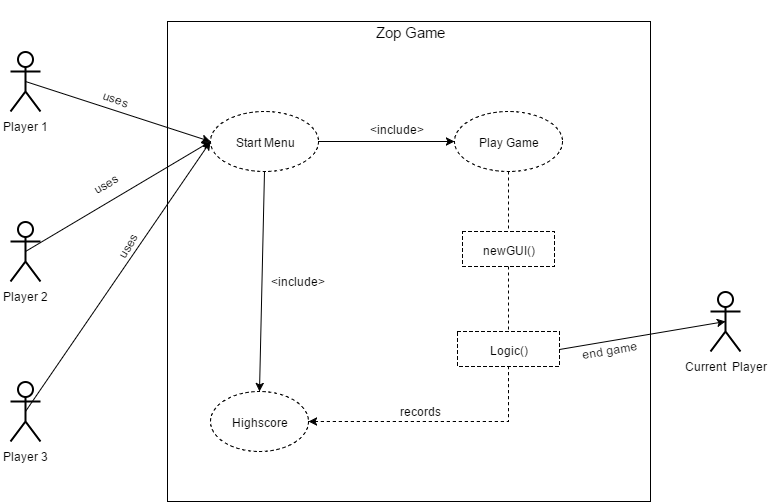
\includegraphics[scale=0.69]{usecase}

\end{document}